\documentclass{beamer}
\usepackage[english]{babel}
\usefonttheme{professionalfonts}
\usepackage{geometry}
\usepackage{amsmath}
\usepackage{amsthm}
\usepackage{graphicx}
\usepackage{caption}
\usepackage[utf8]{inputenc}

%%%%%%%% HYPERREF PACKAGE
\hypersetup{colorlinks=true}
\hypersetup{citecolor=orange}
\hypersetup{urlcolor=orange}

%%%%%%%% DEFINITION AND THEOREM DEFINITIONS
\let\definition\relax
\theoremstyle{definition}
\newtheorem{definition}{Definition}[section]

\let\remark\relax
\theoremstyle{remark}
\newtheorem{remark}{Remark}

\theoremstyle{example}
\newtheorem{question}{Question}

%%%%%%%% MULTI-COLUMNS PACKAGE
\usepackage{multicol}

%%%%%%%% THEME SLIDES
\usetheme{default}

%%%%%%%% BEAMER STUFF
\setbeamertemplate{footline}[frame number]
\setbeamertemplate{section in toc}[sections numbered]
\setbeamertemplate{subsection in toc}[subsections numbered]
\setbeamertemplate{navigation symbols}{}

% Not enumerate frame breaks
% https://tex.stackexchange.com/questions/295854/how-to-edit-behaviour-of-frame-titles-during-frame-break-in-beamer
\setbeamertemplate{frametitle continuation}[from second][]

%%%%%%%% FRAME TITLES AND SUBTITLES
% https://stackoverflow.com/questions/35810906/vim-beamer-dynamic-frame-title1
\newif\ifinsection
\newif\ifinsubsection

\let\oldsection\section
\renewcommand{\section}{
  \global\insectiontrue
  \global\insubsectionfalse
  \oldsection}
\let\oldsubsection\subsection
\renewcommand{\subsection}{
  \global\insubsectiontrue
  \oldsubsection}

\newcommand {\aframe}[1] {
  \begin{frame}
    \ifinsection\frametitle{\secname}\fi
    \ifinsubsection\framesubtitle{\subsecname}\fi
  #1
  \end{frame}
}

% Blue line after title
% https://tex.stackexchange.com/questions/343517/beamer-full-width-hrule-below-frame-title
\setbeamertemplate{frametitle}{%
    \usebeamerfont{frametitle}\insertframetitle\strut%
    \vskip.0\baselineskip%
    \leaders\vrule width 0.85\paperwidth\vskip0.4pt%
    \vskip2pt%
    \usebeamerfont{framesubtitle}\insertframesubtitle
}

%%%%%%%% FOOTNOTE STUFF
\renewcommand{\thefootnote}{\fnsymbol{footnote}}
% Footnote without symbol
% https://tex.stackexchange.com/questions/30720/footnote-without-a-marker
\newcommand\blfootnote[1]{%
  \begingroup
  \renewcommand\thefootnote{}\footnote{#1}%
  \addtocounter{footnote}{-1}%
  \endgroup
}

%%%%%%%% CENTER OF SLIDE THANK YOU
\usepackage{tikz}

%%%%%%%% SETS DEFINITIONS
\usepackage{amssymb}
%%%% Important sets
\renewcommand{\O}{\mathbb{O}}
\newcommand{\N}{\mathbb{N}}
\newcommand{\Z}{{\mathbb{Z}}}
\newcommand{\Q}{{\mathbb{Q}}}
\newcommand{\R}{{\mathbb{R}}}

%%%% Statistics
\newcommand{\E}[1]{\mathbb{E}\left[#1 \right]}
\newcommand{\V}[1]{\mathrm{Var}\left[#1 \right]}

%%%% Lambda Calculus Symbols
\newcommand{\dneq}{\,\, \# \,\,}
\renewcommand{\S}{\pmb{\mathrm{S}}}
\newcommand{\I}{\pmb{\mathrm{I}}}
\newcommand{\K}{\pmb{\mathrm{K}}}
\newcommand{\ch}[1]{\ulcorner #1 \urcorner}

%%%% Make optional parameter
% https://tex.stackexchange.com/questions/217757/special-behavior-if-optional-argument-is-not-passed
\usepackage{xparse}
\NewDocumentCommand{\cx}{o}{
  \IfNoValueTF{#1}
  {\left[\quad\right]}
  {\left[\, #1 \,\right]}
}

%%%%%%%% LOGIC TREES
\usepackage{prftree}

%%%%%%%% SPLIT EQUATIONS
% https://tex.stackexchange.com/questions/51682/is-it-possible-to-pagebreak-aligned-equations
\allowdisplaybreaks

%%%%%%%% TO USE H SPECIFIER
\usepackage{float}

%%%%%%%% TO USE SHORT COMMANDS FOR VECTOR LINES
\usepackage{esvect}

%%%%%%%% START DOCUMENT
\title{Exercise 3.5.2 \textit{i)} - \textit{iii)}}

\author{Juan Sebasti\'an C\'ardenas-Rodríguez \\
  \scalebox{0.7}{Mathematical Engineering, Universidad EAFIT}}

\begin{document}

% Plain so is not numbered
\begin{frame}[plain]
  \titlepage
\end{frame}

%%%%%%%%%% SLIDES %%%%%%%%%%%%%%%
\section{Exercise \textit{i)}}
\subsection{Problem Statement}
\aframe{Find a term with the following $\beta$-graph.
  \begin{figure}[H]
    \centering 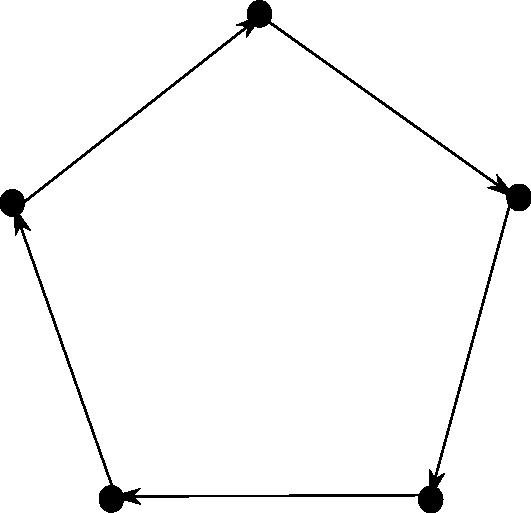
\includegraphics[scale=0.6]{../../graphs/exercise-3-5-2-i.pdf}
  \end{figure}
  Generalize to $n$ vertices. }

\subsection{Pentagon Solution}
\aframe{ Let's define the following lambda terms.
  \begin{equation*}
    R \equiv \lambda abcdf. fabcdf  \quad M \equiv R\I\I\I\I R
  \end{equation*} \pause
  It is clear to see that it reduces in the following manner:
  \begin{align*}
    M &\rightarrow_\beta (\lambda bcdf. f\I bcdf)\I\I\I R \\
      &\rightarrow_\beta (\lambda cdf. f\I\I df)\I\I R \\
      &\rightarrow_\beta (\lambda df. f\I\I\I df)\I R \\
      &\rightarrow_\beta (\lambda f. f\I\I\I\I f) R \\
      &\rightarrow_\beta R\I\I\I\I R \equiv M
  \end{align*}
}

\subsection{Generalization}
\aframe{ For the previous solution, the idea was to generate a term in which
  there was only one possible application each step but, at
  the last one, re-construct the original term. \\
  \vspace{0.3cm}\pause

  Hence, using a similar idea let's define the variables
  $\vv{x_n} \equiv y_0 \ldots y_{n-1}$ and define the sequence of terms as:
  \begin{align*}
    R_0 \equiv y_0 &\quad R_{n+1} \equiv \lambda \vv{x_{n+1}}. (y_{n} \vv{x_{n+1}}) \\
    M_0 \equiv R_0 &\quad M_{n+1} \equiv R_{n+1} \vv{x_n} R_{n+1}
  \end{align*} \pause

  For example for $n=3$, the reduction of $M$ is:
  \begin{align*}
    M_3 \equiv (\lambda y_0y_1y_2. y_2y_0y_1y_2)y_0y_1R_3
    &\rightarrow_\beta (\lambda y_1y_2. y_2y_0y_1y_2)y_1R_3 \\
    &\rightarrow_\beta (\lambda y_2. y_2y_0y_1y_2)R_3 \\
    &\rightarrow_\beta R_3 y_0y_1R_3 \equiv M
  \end{align*}
}

\aframe{ Hence, it is easily seen that for $M_0$ is normal form,
  hence the graph is represented by a vertex with no edges. \pause \\
  \vspace{0.3cm}

  For $M_{n+1}$, the graph would be something like:
  \begin{figure}[H]
    \centering 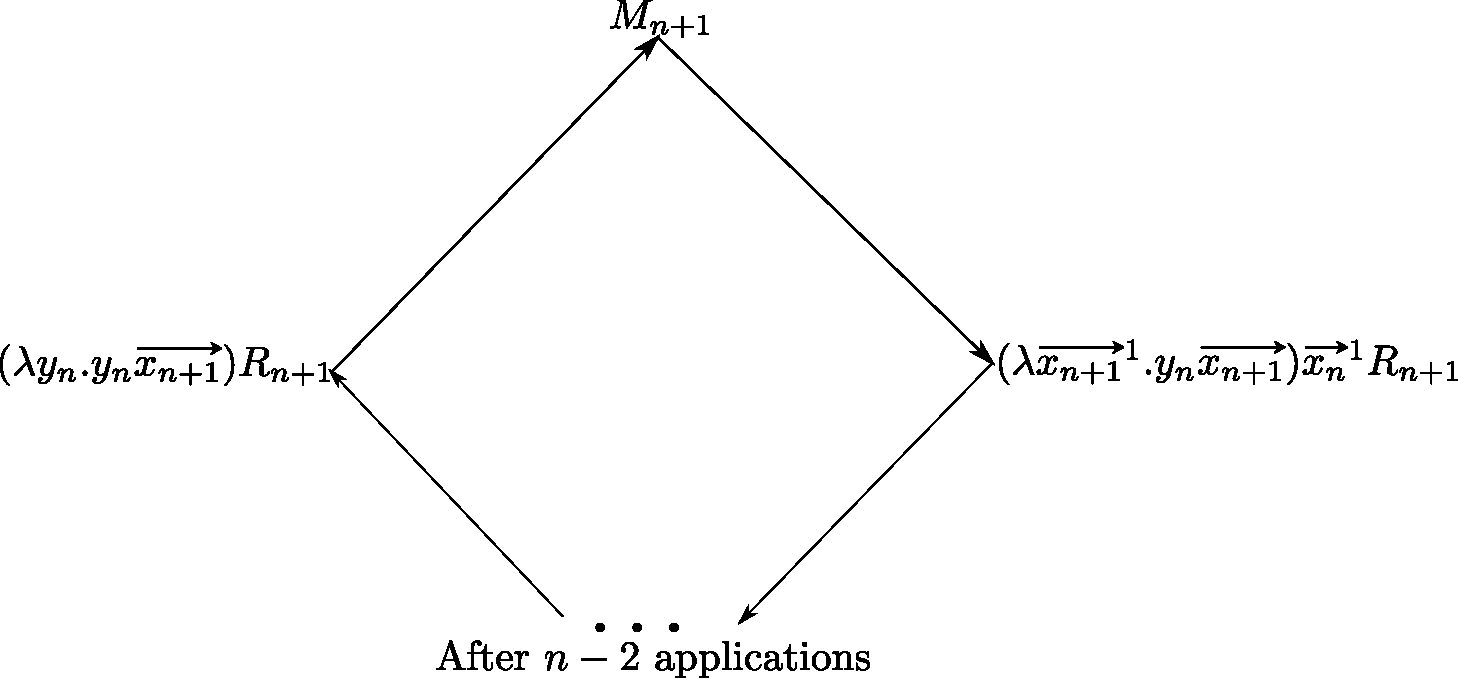
\includegraphics[scale=0.4]{../../graphs/exercise-3-5-2-i-n.pdf}
  \end{figure}
}

\section{Exercise \textit{ii)}}
\subsection{Problem}
\aframe{Find a term that has a reduction graph of
  \begin{figure}[H]
    \centering 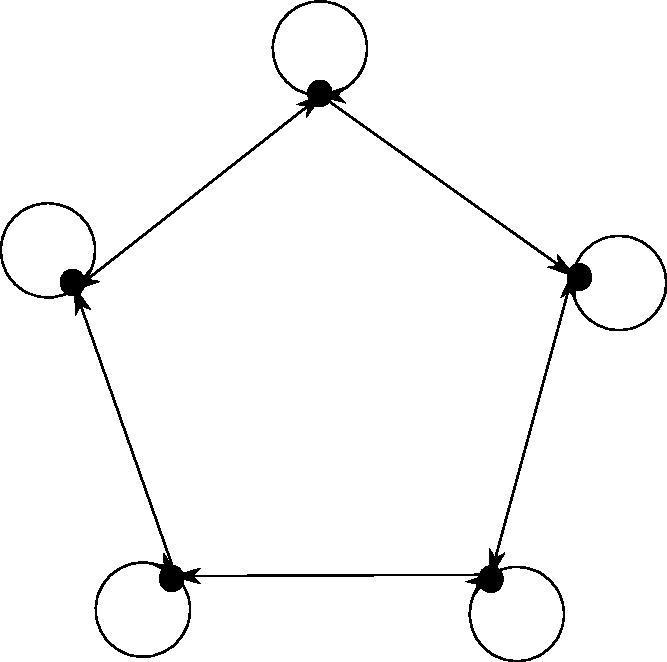
\includegraphics[scale=0.5]{../../graphs/exercise-3-5-2-ii.pdf}
  \end{figure}
}

\subsection{Solution}
\aframe{Remember that $G_\beta(\Omega \equiv (\lambda x. xx)(\lambda x. xx))$
  \begin{figure}[H]
    \centering 
\includegraphics[scale=0.5]{../../graphs/example-omega.pdf}
  \end{figure} \pause \vspace{0.3cm}

  The idea would be to find a term which has two possible applications in each
  step, one in which the term stays the same and another one which advances in
  one direction. \pause \\ \vspace{0.3cm}

  Using the previous problem and $\Omega$ one can define the following term
  which solves the exercise:
  \begin{equation*}
    R \equiv \lambda abcdf. fabcdf  \quad M \equiv \Omega(R \I \I \I \I R)
  \end{equation*}
}

\section{Exercise \textit{iii)}}
\subsection{Problem 1}
\aframe{ Find a term that has a reduction graph of
  \begin{figure}[H]
    \centering
    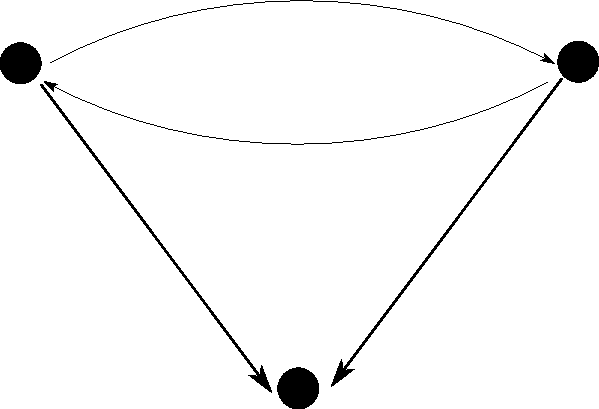
\includegraphics[scale=0.5]{../../graphs/exercise-3-5-2-iii-1.pdf}
  \end{figure}
}

\aframe{ Let's define the terms:
  \begin{equation*}
    W \equiv \lambda xy. yxy \quad M \equiv \K^*(WxW)
  \end{equation*} \pause
  \vspace{0.3cm}
  It is clear to see that the term $M$ reduces in the following manner:
  \begin{alignat*}{2}
    \onslide<3-> {M &\rightarrow_\beta \K^*((\lambda y. yxy)W)} &&
    \onslide<4->{\rightarrow_\beta \K^* (WxW) \equiv M \\}
    \onslide<5-> {&\rightarrow_\beta \I} \onslide<6>{&&\rightarrow_\beta \I}
  \end{alignat*}

  \onslide<3->{
    \begin{figure}[H]
      \centering
      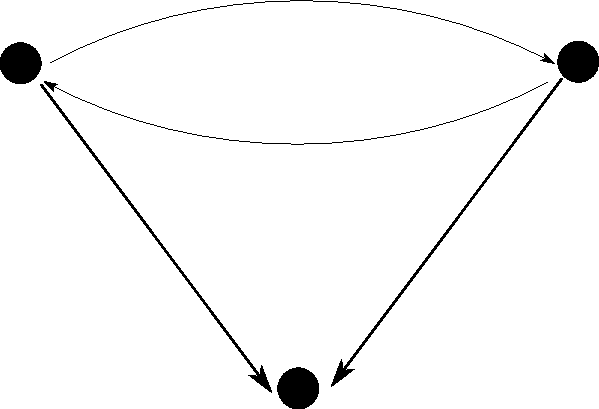
\includegraphics[scale=0.5]{../../graphs/exercise-3-5-2-iii-1.pdf}
    \end{figure}} }

\subsection{Problem 2}
\aframe{ Find a term that has a reduction graph of
  \begin{figure}[H]
    \centering
    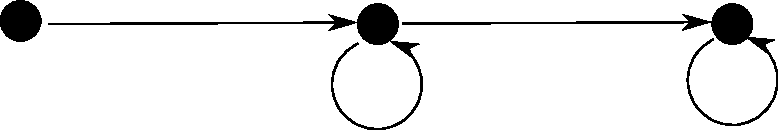
\includegraphics[scale=0.5]{../../graphs/exercise-3-5-2-iii-2.pdf}
  \end{figure}
}

\aframe{ Let's define the terms:
  \begin{equation*}
    M \equiv (\lambda xy. xx) (\lambda z. zz) y
  \end{equation*} \pause
  \vspace{0.3cm}
  It is clear to see that the term $M$ reduces in the following manner:
  \begin{align*}
    \onslide<3-> { M \rightarrow_\beta (\lambda y. \Omega) y} &
                                                                \onslide<4->{\rightarrow_\beta \Omega \\}
    \onslide<5->{&\rightarrow_\beta (\lambda y. \Omega) y}
  \end{align*}

  \onslide<3->{
    \begin{figure}[H]
      \centering
      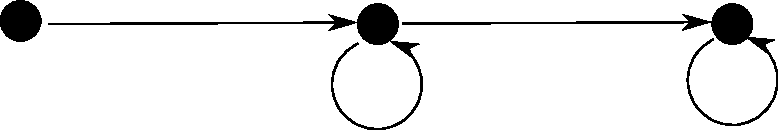
\includegraphics[scale=0.5]{../../graphs/exercise-3-5-2-iii-2.pdf}
    \end{figure}} }

\subsection{Problem 3}
\aframe{ Find a term that has a reduction graph of
  \begin{figure}[H]
    \centering
    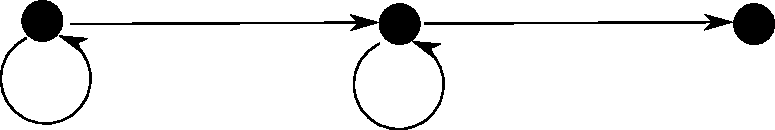
\includegraphics[scale=0.5]{../../graphs/exercise-3-5-2-iii-3.pdf}
  \end{figure}
}

\aframe{ Let's define the terms:
  \begin{equation*}
    M \equiv (\lambda y. y\Omega)(\lambda x. y)
  \end{equation*} \pause
  \vspace{0.3cm}
  It is clear to see that the term $M$ reduces in the following manner:
  \begin{alignat*}{2}
    \onslide<3->{M &\rightarrow_\beta \qquad
      \,\,(\lambda x. y)\Omega} \onslide<4->{&&\rightarrow_\beta y \\}
    \onslide<5->{&\rightarrow_\beta (\lambda y. y\Omega)(\lambda x.y) \equiv M}&& \\
    & \onslide<6>{&&\rightarrow_\beta (\lambda x. y)\Omega}
  \end{alignat*}

  \onslide<3->{
    \begin{figure}[H]
      \centering
      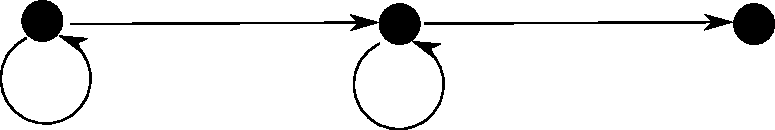
\includegraphics[scale=0.5]{../../graphs/exercise-3-5-2-iii-3.pdf}
    \end{figure}} }

%%%%%%%%%%%%%%%%%%%%%%%%%%%%%%%%%
\begin{frame}
  \begin{tikzpicture}[overlay, remember picture]
    \node[anchor=center] at (current page.center) { \Huge{\emph{Thank you!}}};
  \end{tikzpicture}
  \begin{minipage}[t][.8\textheight]{\textwidth}
    \vfill
    \begin{center}
      \scalebox{0.7}{Juan Sebasti\'an C\'ardenas-Rodríguez} \\
      \scalebox{0.7}{jscardenar@eafit.edu.co} \\
    \end{center}
  \end{minipage}
\end{frame}

\end{document}
